\chapter{Biología estructural de las proteínas}\label{ch:b3:structural-biology}

Max Perutz empezó a trabajar en la estructura de la hemoglobina en 1937 y
la publicó en 1960: veintidós años para ver, con una \omterm{def:b3:structural-biology:methods}{resolución} de medio
nanómetro, cómo cuatro cadenas de ciento cincuenta aminoácidos se pliegan
en torno a cuatro hemos. Una molécula de hemoglobina se pliega sola en
unos pocos milisegundos. Entre estos dos hechos está el asunto de este
capítulo: qué es la forma de una proteína, por qué una cadena de
aminoácidos tiene una forma y no otra, cómo la encuentra tan deprisa
entre un número astronómico de alternativas, qué falla cuando no lo hace,
cómo se ven las formas --- con rayos X, con resonancia magnética, con
electrones y ahora con cálculo --- y cómo una proteína se mueve entre
formas para hacer su trabajo, con el conmutador de la hemoglobina entre
una forma tensa y otra relajada como modelo de toda proteína alostérica
desde entonces.

\section{Qué es la estructura de una proteína}

\begin{definition}[Niveles de estructura]\label{def:b3:structural-biology:levels}
\index{estructura secundaria}\index{hélice alfa}\index{lámina beta}\index{estructura terciaria}\index{dominio}\index{plegamiento}
La \emph{estructura primaria} es la secuencia de residuos. La
\emph{estructura secundaria} es la conformación regular local del
esqueleto, estabilizada por puentes de hidrógeno entre los carbonilos y
las amidas del esqueleto: la \emph{hélice~$\alpha$}, una espiral dextrógira
de $3.6$ residuos por vuelta que sube \qty{0.15}{nm} por residuo
(\qty{0.54}{nm} por vuelta), con cada carbonilo unido a la amida situada
cuatro residuos más allá; y la \emph{lámina~$\beta$}, en la que hebras
extendidas se disponen lado a lado, paralelas o antiparalelas, unidas a
sus vecinas, con las cadenas laterales alternando por encima y por debajo
de la lámina. La \emph{estructura terciaria} es el plegamiento de toda
una cadena en tres dimensiones; una unidad compacta de \numrange{50}{250}
residuos que se pliega de forma independiente dentro de ella es un
\emph{dominio}, y la disposición de los elementos secundarios de un
dominio es su \emph{plegamiento}. La \emph{estructura cuaternaria} es el
ensamblaje de varias cadenas: el $\alpha_{2}\beta_{2}$ de la hemoglobina.
Unos \num{1300} plegamientos dan cuenta de todos los dominios conocidos,
y unas pocas decenas de ellos --- el plegamiento de Rossmann, el barril
TIM, el plegamiento de las inmunoglobulinas --- de una gran parte de
todas las proteínas: la naturaleza reutiliza plegamientos y varía sus
secuencias.
\end{definition}

\begin{omfigure}
\begin{tikzpicture}
\begin{axis}[
  width=6.4cm, height=6.4cm,
  xmin=-180, xmax=180, ymin=-180, ymax=180,
  xlabel={$\phi$ (grados)}, ylabel={$\psi$ (grados)},
  xlabel style={font=\small}, ylabel style={font=\small},
  tick label style={font=\scriptsize}, xtick={-180,-90,0,90,180}, ytick={-180,-90,0,90,180},
  axis lines=box, grid=major, grid style={gray!25},
  clip=false,
]
% beta region
\fill[omDef!30] (axis cs:-180,90) rectangle (axis cs:-45,180);
\fill[omDef!30] (axis cs:-180,-180) rectangle (axis cs:-45,-150);
\node[font=\scriptsize, omDef!60!black] at (axis cs:-112,165) {hebras $\beta$};
% alpha R region
\fill[omThm!30] (axis cs:-160,-70) rectangle (axis cs:-45,0);
\node[font=\scriptsize, omThm!70!black] at (axis cs:-105,-58) {$\alpha$ dextrógira};
% alpha L region
\fill[omMeth!30] (axis cs:45,0) rectangle (axis cs:100,80);
\node[font=\scriptsize, omMeth!60!black, align=center] at (axis cs:72,40) {levógira};
\addplot[only marks, mark=*, mark size=1pt, black] coordinates {(-57,-47)};
\node[font=\scriptsize, anchor=south west] at (axis cs:-52,-44) {$\alpha$: $(-57,-47)$};
\addplot[only marks, mark=*, mark size=1pt, black] coordinates {(-139,135)};
\node[font=\scriptsize, anchor=west] at (axis cs:-134,135) {$\beta$ antiparalela};
\end{axis}
\node[align=left, font=\scriptsize, anchor=west] at (7.0,3.0) {Los dos ángulos de torsión del esqueleto de\\cada residuo, $\phi$ (en torno a N--C$_\alpha$) y $\psi$ (en\\torno a C$_\alpha$--C), están restringidos por choques\\estéricos a las regiones coloreadas. Una\\hélice pone todos los residuos en un punto; una\\hebra, cerca de otro. La glicina, sin cadena lateral,\\llega más lejos; la prolina, con su anillo, queda\\fija cerca de $\phi = -60$.};
\end{tikzpicture}

{\small El diagrama de Ramachandran. Las regiones sombreadas son las
combinaciones de los ángulos $\phi$ y $\psi$ del esqueleto permitidas
estéricamente; la hélice~$\alpha$ dextrógira y la hebra~$\beta$
corresponden cada una a una región pequeña, y la mayoría de los residuos
de una proteína plegada caen en una de ellas.}
\end{omfigure}

\begin{proposition}[Qué mantiene unido un plegamiento]\label{prop:b3:structural-biology:forces}
\index{efecto hidrófobo}\index{estabilidad marginal}
Una proteína plegada la estabilizan el \emph{\omterm{prop:b3:structural-biology:forces}{efecto hidrófobo}} ---
enterrar las cadenas laterales apolares en un núcleo lejos del agua, lo
que libera las moléculas de agua que de otro modo quedarían ordenadas a
su alrededor ---, los puentes de hidrógeno de la \omterm{def:b3:structural-biology:levels}{estructura secundaria} y
de los grupos polares enterrados, el empaquetamiento de van der Waals de
un núcleo tan denso como un cristal, algún que otro puente salino y, en
las proteínas secretadas, los puentes disulfuro. El \omterm{prop:b3:structural-biology:forces}{efecto hidrófobo}
aporta la mayor parte del impulso; los puentes de hidrógeno se pagan
sobre todo a sí mismos (un esqueleto unido al agua en el estado
desplegado queda unido a sí mismo en el plegado) y lo que dictan es
\emph{cuál} es el \omterm{def:b3:structural-biology:levels}{plegamiento}. La energía libre neta del \omterm{def:b3:structural-biology:levels}{plegamiento} es
pequeña, $\Delta G \approx -20$ a \qty{-60}{kJ/mol} --- la fuerza de un
puñado de puentes de hidrógeno en una molécula que tiene centenares ---,
porque la pérdida de entropía conformacional al plegarse casi cancela la
ganancia de entalpía. Las proteínas son de \emph{\omterm{prop:b3:structural-biology:forces}{estabilidad marginal}}:
unos pocos grados, un cambio de pH o una sola mutación en el núcleo
pueden desplegarlas, y esa marginalidad es lo que les permite moverse.
\end{proposition}

\begin{proof}[Evidencia]
Anfinsen (1961) desplegó la ribonucleasa~A con urea y un agente reductor,
rompió sus cuatro puentes disulfuro y destruyó su actividad; al quitar
ambos, la enzima se replegó, volvió a formar los cuatro emparejamientos
correctos de entre los $105$ posibles y recuperó toda su actividad. No
había molde, ni enzima, ni más información que la secuencia: la
estructura nativa es el estado termodinámicamente más estable accesible a
la cadena, y la secuencia la codifica. Reoxidar los puentes disulfuro
mientras la cadena seguía en urea dio una mezcla desordenada con un
\qty{1}{\%} de actividad, que después se ordenó hasta la forma nativa
cuando se la dejó plegarse: la cadena encuentra el mínimo por sí sola.
\end{proof}

\section{Cómo encuentra una cadena su plegamiento}

\begin{theorem}[La paradoja de Levinthal]\label{thm:b3:structural-biology:levinthal}
\index{paradoja de Levinthal}\index{embudo de plegamiento}
Si cada uno de los $n$ residuos de una proteína pudiera adoptar $k$
conformaciones de esqueleto de forma independiente, la cadena tendría
$k^{n}$ conformaciones. Con $k = 3$ y $n = 100$ eso son $3^{100} \approx
5\times 10^{47}$; muestrearlas a una por picosegundo ($10^{12}$ por
segundo) costaría $5\times 10^{35}$ segundos, unos $10^{28}$ años. Las
proteínas de ese tamaño se pliegan en milisegundos o segundos. Por tanto
el \omterm{def:b3:structural-biology:levels}{plegamiento} no es una búsqueda al azar entre conformaciones: la
superficie de energía es un \emph{embudo} en el que casi toda
conformación parcial está sesgada hacia el estado nativo, y la cadena
desciende mediante movimientos locales que en promedio van cuesta abajo.
\end{theorem}
\begin{proof}
El recuento es el principio de multiplicación; el tiempo es el recuento
dividido por la velocidad de muestreo, $5\times 10^{47}/10^{12} = 5\times
10^{35}$ s, y un año son $3\times 10^{7}$ s. La conclusión es el
contrarrecíproco: una búsqueda al azar de ese tamaño es imposible en el
tiempo observado, luego la búsqueda no es al azar. Lo que la hace no
aleatoria es que una interacción formada en una parte de la cadena
persiste mientras se forman otras (el colapso hidrófobo y la formación de
hélices ocurren en microsegundos y reducen el espacio que hay que
explorar), y que las estructuras parcialmente correctas tienen en
promedio menos energía que las erróneas, de modo que el descenso está
guiado --- un embudo y no un campo de golf con un solo hoyo.
\end{proof}

\begin{omfigure}
\begin{tikzpicture}[every node/.style={font=\scriptsize}, >=stealth]
  % funnel outline
  \draw[very thick, omDef] (-4,3) .. controls (-3.2,1.5) and (-1.2,0.2) .. (-0.35,-1.2) -- (-0.35,-1.6);
  \draw[very thick, omDef] (4,3) .. controls (3.2,1.5) and (1.2,0.2) .. (0.35,-1.2) -- (0.35,-1.6);
  \draw[very thick, omDef] (-0.35,-1.6) -- (0.35,-1.6);
  % rugged inner lines
  \draw[omDef!60, thick] (-3.3,2.6) .. controls (-2.9,2.2) and (-2.6,2.6) .. (-2.2,2.0) .. controls (-1.9,1.5) and (-1.7,1.9) .. (-1.4,1.2) .. controls (-1.1,0.7) and (-0.9,0.9) .. (-0.6,0.2);
  \draw[omDef!60, thick] (3.3,2.6) .. controls (2.9,2.1) and (2.5,2.5) .. (2.1,1.8) .. controls (1.8,1.3) and (1.5,1.6) .. (1.2,1.0) .. controls (1.0,0.6) and (0.8,0.8) .. (0.6,0.2);
  % axes
  \draw[->] (-5.9,-1.8) -- (-5.9,3.2) node[above, align=center] {energía\\libre};
  \draw[<->] (-3.9,3.85) -- (3.9,3.85) node[midway, above] {entropía conformacional (amplitud del conjunto)};
  % labels
  \node[above] at (0,3.05) {cadena desplegada: muchas conformaciones, energía alta};
  \node[right, align=left] at (3.3,1.4) {trampas locales: intermediarios\\mal plegados en parte};
  \node[left, align=right] at (-3.3,1.4) {colapso rápido y\\estructura secundaria};
  \node[below] at (0,-1.7) {estado nativo: una conformación, la energía más baja};
  \draw[->, thick, omThm] (-2.8,2.4) .. controls (-2.0,1.2) and (-0.8,0.5) .. (-0.15,-1.3);
  \node[omThm, left] at (-1.5,-0.5) {una trayectoria de plegamiento};
\end{tikzpicture}

{\small El \omterm{thm:b3:structural-biology:levinthal}{embudo de plegamiento}. La energía libre cae y el número de
conformaciones disponibles se encoge a medida que la cadena se acerca al
estado nativo; las paredes son rugosas, de modo que una cadena puede
quedar atrapada en un intermediario mal plegado en parte, pero la
pendiente global la lleva abajo en milisegundos.}
\end{omfigure}

\begin{definition}[Chaperonas]\label{def:b3:structural-biology:chaperones}
\index{chaperona}\index{Hsp70}\index{chaperonina}\index{GroEL}
Una \emph{chaperona molecular} es una proteína que ayuda al \omterm{def:b3:structural-biology:levels}{plegamiento}
de otras sin formar parte de ellas ni aportar información sobre el
\omterm{def:b3:structural-biology:levels}{plegamiento}: impide la agregación que compite con el \omterm{def:b3:structural-biology:levels}{plegamiento} en el
citoplasma abarrotado. La \emph{Hsp70} se une a segmentos hidrófobos
expuestos de cadenas nacientes o desplegadas y los suelta al hidrolizar
ATP para otro intento; la \emph{chaperonina} GroEL (Hsp60 en las
mitocondrias, TRiC en el citosol eucariota) es un barril doble de catorce
subunidades cuya cavidad central, tapada por GroES, encierra en
aislamiento una sola cadena de hasta \qty{60}{kDa} durante unos diez
segundos --- una jaula de Anfinsen --- y la expulsa esté plegada o no,
para que lo intente de nuevo. Cerca de la décima parte de las proteínas
bacterianas recién fabricadas pasan por GroEL, y una célula cuyas
chaperonas se ven desbordadas --- por el calor, que es por lo que la
mayoría son \emph{proteínas de choque térmico} inducidas por una subida
de temperatura --- se llena de agregados.
\end{definition}

\begin{definition}[Amiloide]\label{def:b3:structural-biology:amyloid}
\index{amiloide}\index{beta cruzada}\index{prion}\index{enfermedad por mal plegamiento}
El \emph{amiloide} es un agregado ordenado de proteína en el que las
cadenas se apilan en fibrillas no ramificadas de \qtyrange{5}{10}{nm} de
ancho, con las hebras de cada cadena perpendiculares al eje de la
fibrilla y unidas por puentes de hidrógeno a las hebras de la siguiente
--- la estructura \emph{$\beta$ cruzada}, la misma sea cual sea la
proteína. Casi cualquier proteína puede formarlo en condiciones
desestabilizadoras; en las \emph{enfermedades por mal \omterm{def:b3:structural-biology:levels}{plegamiento}} lo
hacen en el cuerpo proteínas concretas: el amiloide~$\beta$ y la tau en
la enfermedad de Alzheimer, la $\alpha$-sinucleína en la de Parkinson, la
huntingtina, la transtiretina y el amiloide de los islotes en la diabetes
de tipo~2. Un \emph{prion} es un amiloide que se propaga: la forma mal
plegada de la proteína priónica PrP convierte por contacto la forma
normal en más de sí misma, de modo que la ``infección'' no lleva ácido
nucleico alguno, solo una forma --- el mecanismo de la tembladera, de la
encefalopatía espongiforme bovina y de la enfermedad de
Creutzfeldt--Jakob, establecido por Prusiner desde 1982 contra una larga
resistencia.
\end{definition}

\begin{omfigure}
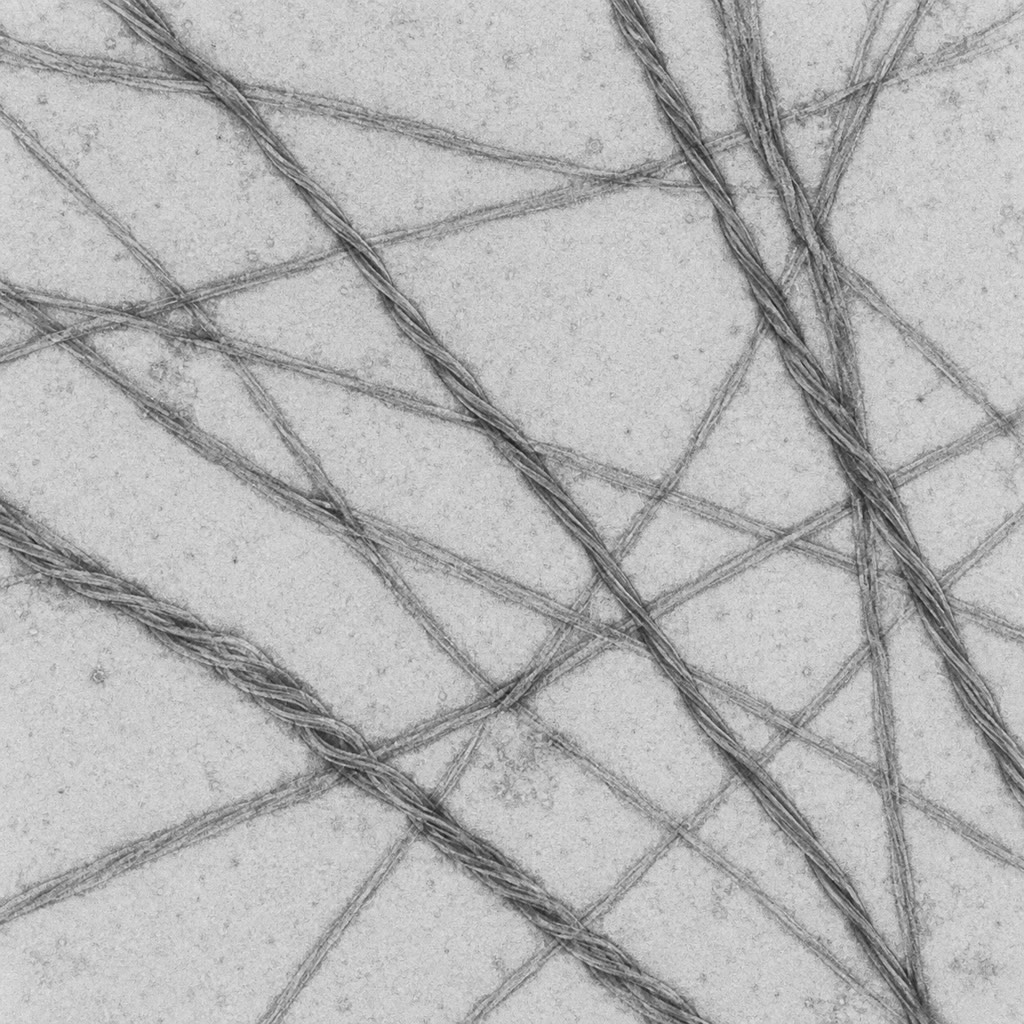
\includegraphics[width=0.36\linewidth]{images/book5/ai/b5-07-amyloid-fibrils.jpg}\hspace{0.04\linewidth}
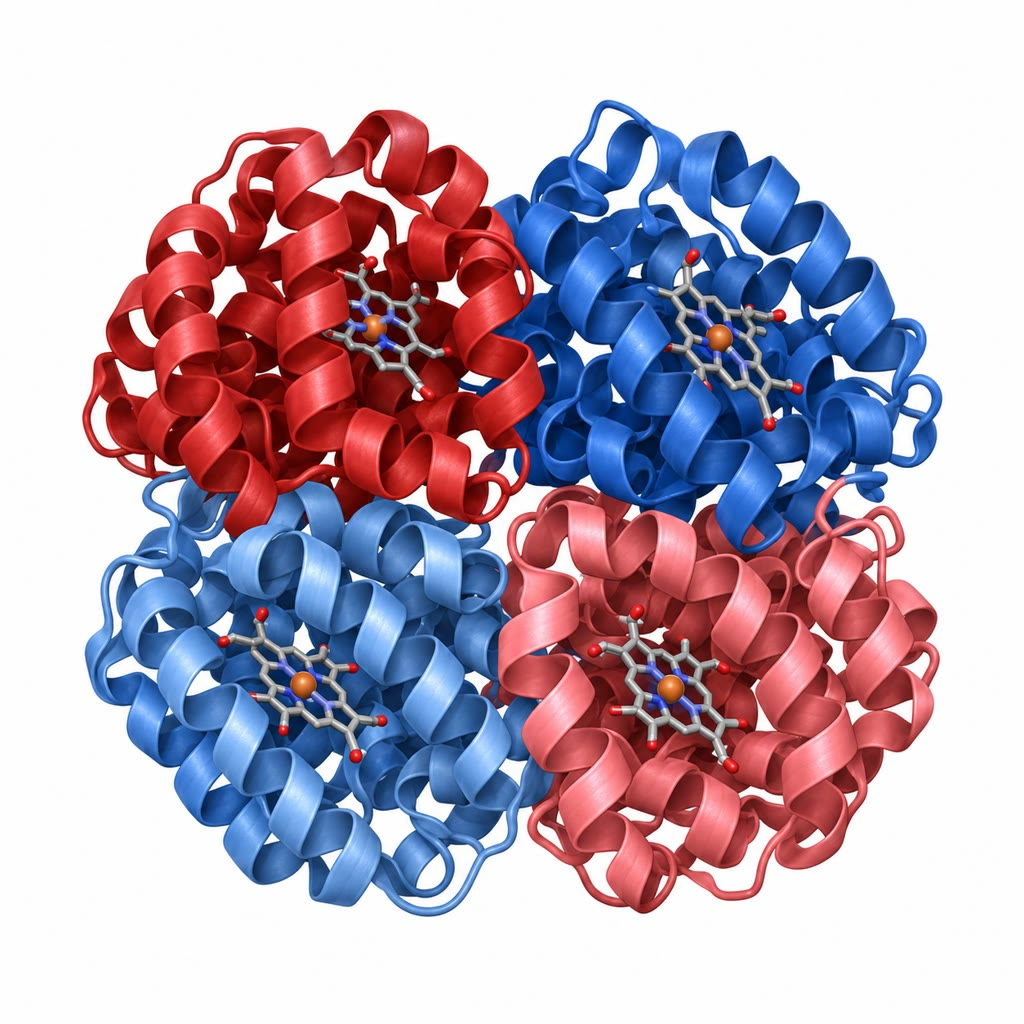
\includegraphics[width=0.36\linewidth]{images/book5/ai/b5-07-haemoglobin-model.jpg}

{\small Izquierda: fibrillas de \omterm{def:b3:structural-biology:amyloid}{amiloide} al microscopio electrónico ---
rectas, no ramificadas, a veces retorcidas y estructuralmente parecidas
sea cual sea la proteína de la que estén hechas. Derecha: el tetrámero de
la hemoglobina, dos cadenas $\alpha$ y dos $\beta$, cada una acunando un
hemo.}
\end{omfigure}

\section{Ver una proteína}

\begin{definition}[Métodos estructurales]\label{def:b3:structural-biology:methods}
\index{cristalografía de rayos X}\index{espectroscopia de RMN}\index{criomicroscopia electrónica}\index{resolución}
La \emph{cristalografía de rayos X} hace crecer un cristal de la
proteína, lo expone a un haz de rayos X y registra el patrón de
difracción; las posiciones de las manchas dan la red, y sus intensidades,
una vez recuperadas las fases de las ondas, dan la densidad electrónica
de la celda unidad, dentro de la cual se construye la cadena. La
\emph{resonancia magnética nuclear} (RMN) mide, en disolución, los
acoplamientos entre los núcleos de átomos próximos en el espacio, de los
que se calculan distancias y con ellas una estructura; sirve para
proteínas de menos de unos \qty{40}{kDa} e informa de sus movimientos. La
\emph{criomicroscopia electrónica} fotografía de miles a millones de
moléculas sueltas congeladas en una película fina de hielo vítreo, cada
una en una orientación al azar, y reconstruye la densidad tridimensional
combinándolas; desde los detectores directos de electrones (2013) alcanza
resolución atómica y no necesita cristal, de modo que hoy se resuelven de
rutina grandes complejos, proteínas de membrana y ensamblajes flexibles
que nunca cristalizaron. La \emph{resolución} de una estructura es la
menor separación a la que dos rasgos quedan distinguidos: a
\qty{0.35}{nm} se sitúan el esqueleto y las cadenas laterales grandes, a
\qty{0.2}{nm} todos los átomos y a \qty{0.1}{nm} los hidrógenos.
\end{definition}

\begin{proof}[Evidencia]
Kendrew (1958) obtuvo la primera estructura de una proteína, la
mioglobina de cachalote, a \qty{0.6}{nm} --- una salchicha de una
irregularidad inesperada, ``más complicada y menos simétrica de lo que
nadie había predicho'' --- y a \qty{0.2}{nm} en 1960, cuando se vieron
por primera vez las hélices~$\alpha$ que Pauling había propuesto
construyendo modelos en 1951. Perutz (1960) resolvió la hemoglobina a
\qty{0.55}{nm} usando el método de átomos pesados que había ideado para
obtener las fases: unos átomos de mercurio unidos a la proteína cambian
las intensidades de un modo que revela la información que falta.
Comparando las formas oxigenada y desoxigenada (1970) vio que las
subunidades giran unas contra otras \qty{15}{\degree} al unir oxígeno, la
primera transición alostérica observada a escala atómica.
\end{proof}

\begin{omfigure}
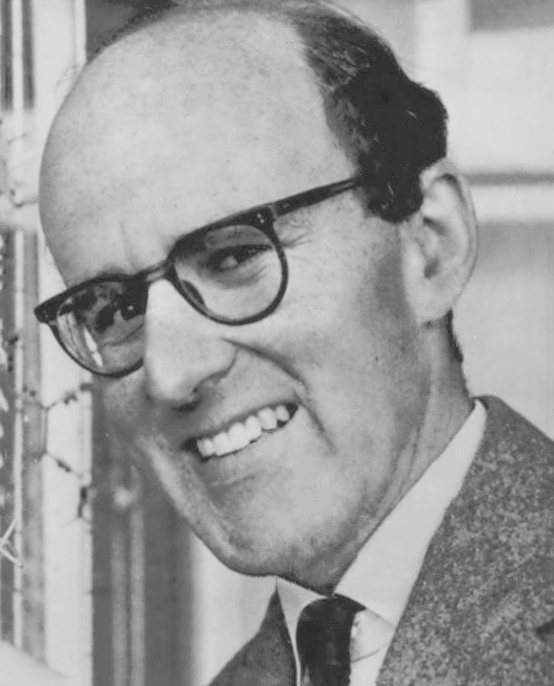
\includegraphics[width=0.30\linewidth]{images/book5/perutz.jpg}\hspace{0.04\linewidth}
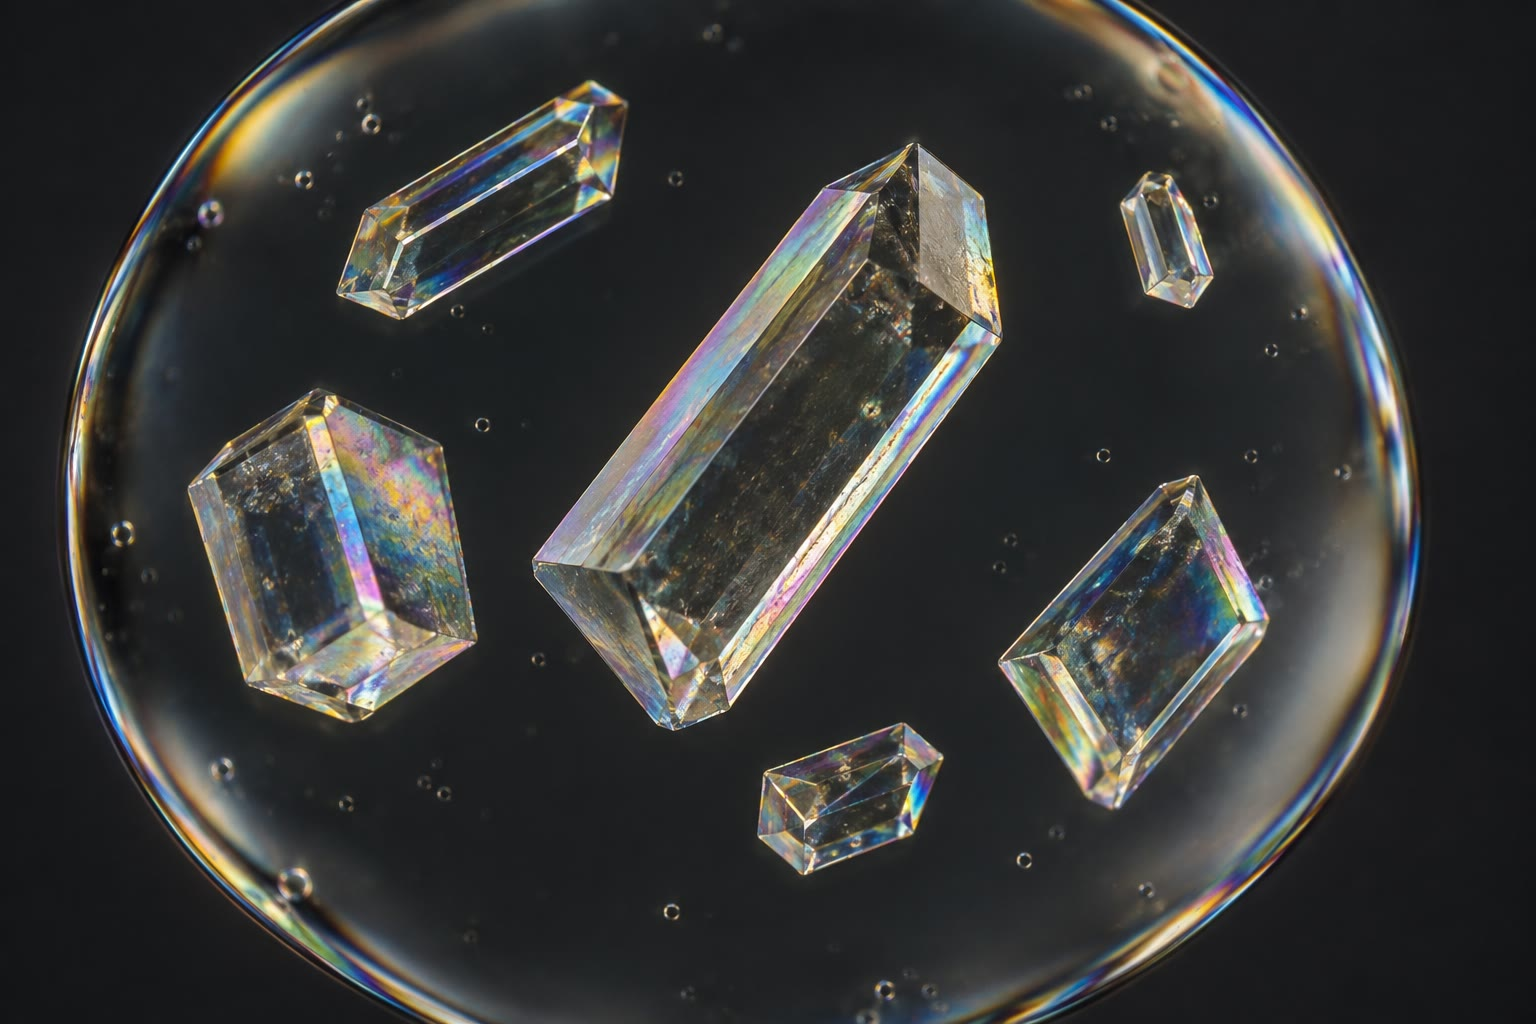
\includegraphics[width=0.30\linewidth]{images/book5/ai/b5-07-protein-crystals.jpg}\hspace{0.04\linewidth}
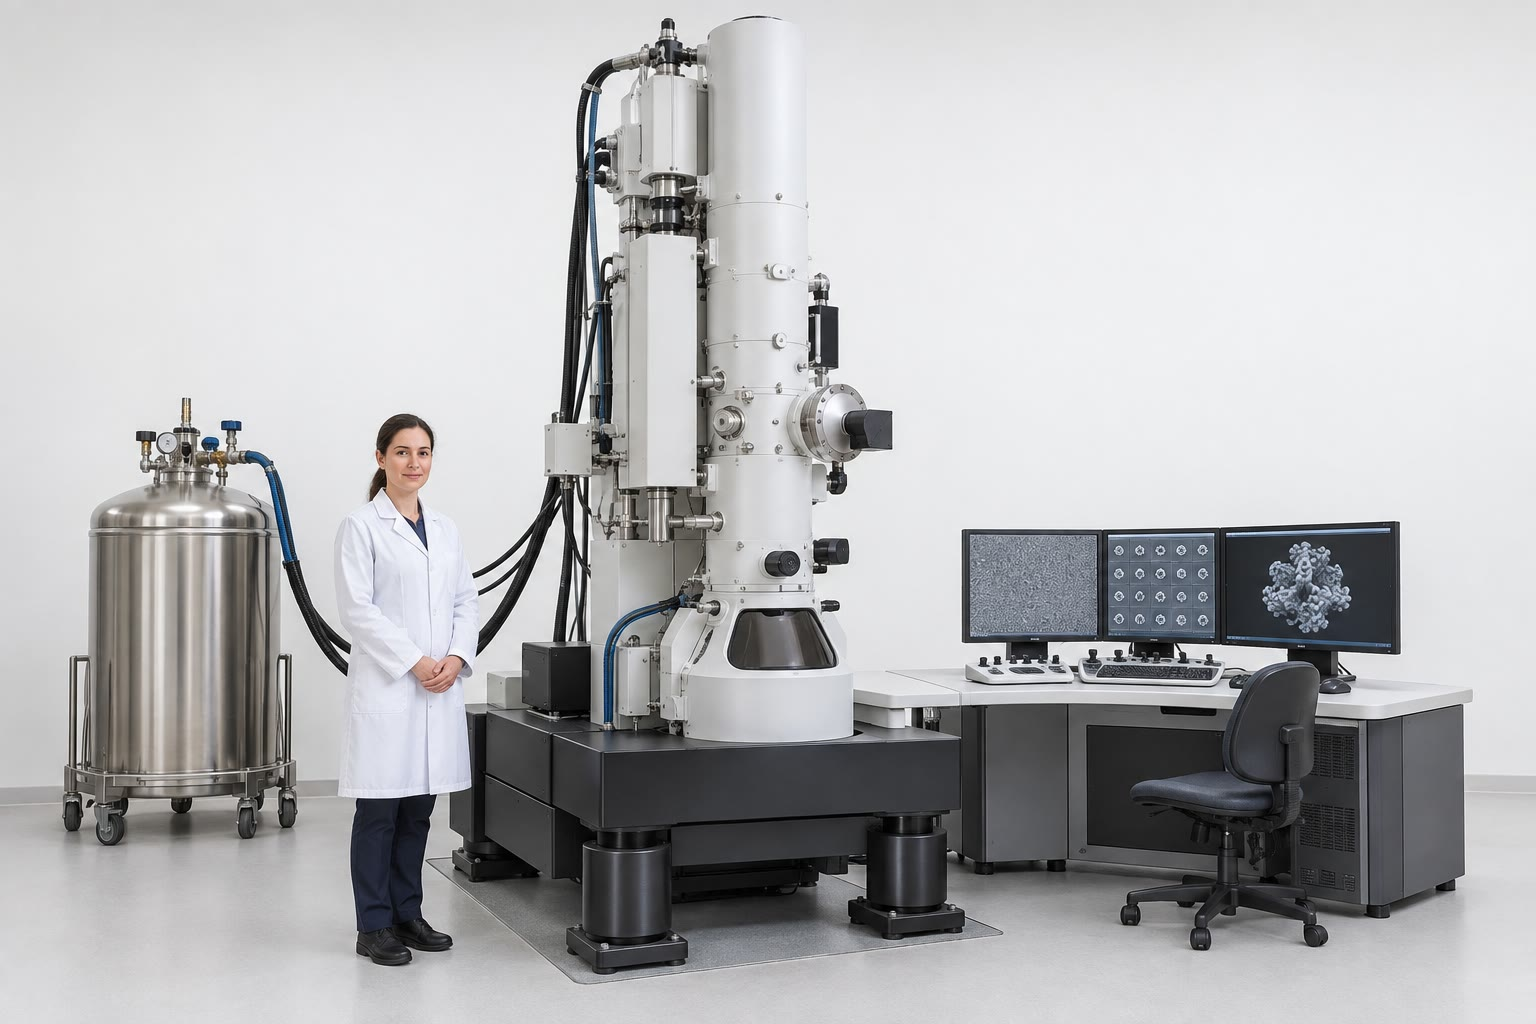
\includegraphics[width=0.30\linewidth]{images/book5/ai/b5-07-cryo-em.jpg}

{\small Max Perutz en 1962, el año de su premio Nobel por la estructura
de la hemoglobina (Associated Press, \omterm{def:b3:structural-biology:levels}{dominio} público). Centro: cristales
de proteína en una gota colgante, el punto de partida de la
cristalografía. Derecha: un criomicroscopio electrónico, el instrumento
que hizo innecesarios los cristales.}
\end{omfigure}

\begin{method}[Resolver una estructura por cristalografía]\label{met:b3:structural-biology:crystallography}
\index{ley de Bragg}\index{problema de las fases}
(1) Purifíquense miligramos de la proteína y críbense centenares de
condiciones (precipitante, pH, sal) buscando cristales; (2) congélese de
golpe un cristal y recójanse imágenes de difracción en un sincrotrón
mientras gira en el haz; (3) indícense las manchas para obtener la celda
unidad y la simetría; el ángulo mayor al que se ven manchas fija la
\omterm{def:b3:structural-biology:methods}{resolución} por la \omterm{met:b3:structural-biology:crystallography}{ley de Bragg}, $d =
\lambda/(2\sin\theta)$; (4) resuélvase el \emph{problema de las fases}
--- el detector registra intensidades pero no fases --- con átomos
pesados, con la dispersión anómala del selenio de la selenometionina o,
para una proteína parecida a otra conocida, por sustitución molecular,
colocando el modelo conocido en la celda; (5) calcúlese la densidad
electrónica, constrúyase la cadena dentro de ella y refínese el modelo
contra los datos hasta que el desacuerdo (el factor $R$) sea pequeño;
(6) valídese: geometría, valores atípicos de Ramachandran y el ajuste a
datos contra los que el modelo no se refinó.
\end{method}

\begin{omfigure}
\begin{tikzpicture}[every node/.style={font=\scriptsize}, >=stealth]
  % crystal
  \draw[thick, fill=omDef!20] (0,0) -- (1.4,0) -- (1.9,0.6) -- (0.5,0.6) -- cycle; \draw[thick, fill=omDef!30] (0,0) -- (0.5,0.6) -- (0.5,1.6) -- (0,1.0) -- cycle; \draw[thick, fill=omDef!25] (0.5,0.6) -- (1.9,0.6) -- (1.9,1.6) -- (0.5,1.6) -- cycle;
  \node[below] at (0.95,-0.1) {cristal: $10^{12}$ moléculas alineadas};
  % beam
  \draw[->, very thick, omThm] (-2.2,0.9) -- (-0.1,0.9); \node[above] at (-1.2,0.95) {rayos X, $\lambda \approx \qty{0.1}{nm}$};
  % diffracted beams
  \foreach \a in {-25,-12,5,18,30} \draw[->, omThm, thick] (1.9,0.9) -- ++(\a:3.2);
  % detector
  \draw[thick] (5.2,-1.2) rectangle (5.6,3.0); \node[right, align=left] at (5.7,2.6) {detector: manchas a\\ángulos $\theta$, con\\intensidades $I$};
  \foreach \y in {-0.6,-0.1,0.6,1.2,1.9,2.4} \fill[black] (5.4,\y) circle (0.06);
  % arrow to density
  \draw[->, very thick] (7.4,0.9) -- (8.6,0.9) node[midway, above, align=center] {fases\\recuperadas};
  \node[right, align=left] at (8.7,1.4) {densidad electrónica};
  \draw[omDef, thick] (8.8,0.4) .. controls (9.1,1.1) and (9.5,0.2) .. (9.8,0.8) .. controls (10.1,1.3) and (10.4,0.3) .. (10.7,0.9);
  \node[right, align=left] at (8.7,-0.4) {modelo construido dentro,\\refinado, validado};
  % Bragg
  \node[anchor=north west, align=left] at (-2.2,-0.7) {Bragg: $2d\sin\theta = \lambda$ ---\\el mayor $\theta$ observado fija la resolución $d$};
\end{tikzpicture}

{\small Del cristal al modelo. La red regular dispersa los rayos X en
manchas discretas; la mancha situada al ángulo mayor fija la \omterm{def:b3:structural-biology:methods}{resolución};
recuperar las fases convierte las intensidades en un mapa de densidad
electrónica, dentro del cual se construye la cadena.}
\end{omfigure}

\begin{remark}[La predicción se ha sumado a los métodos]\label{rem:b3:structural-biology:prediction}
Desde 2020 la estructura de una proteína se predice a partir de su
secuencia con una exactitud que a menudo rivaliza con una estructura
experimental de \qty{0.3}{nm} (\cref{ch:b3:bioinformatics}). La
predicción es una hipótesis sobre un estado nativo estático; los métodos
experimentales siguen siendo el árbitro y la única fuente de información
sobre ligandos, cambios conformacionales, complejos y la dinámica de más
abajo. Sus papeles han cambiado --- un modelo predicho resuelve el
problema de las fases por sustitución molecular y orienta qué
experimentos vale la pena hacer --- más que sustituirse el uno al otro.
\end{remark}

\section{Alosterismo: la hemoglobina como modelo}

\begin{definition}[Alosterismo y cooperatividad]\label{def:b3:structural-biology:allostery}
\index{alosterismo}\index{cooperatividad}\index{coeficiente de Hill}\index{estado T}\index{estado R}
Una proteína es \emph{alostérica} cuando la unión de un ligando en un
sitio cambia la afinidad de otro, mediante un cambio de conformación
transmitido a través de la molécula. Cuando los dos sitios unen el mismo
ligando y el efecto es positivo, la unión es \emph{cooperativa}: la
saturación fraccionaria $Y$ sube con la concentración de ligando como una
sigmoide y no como una hipérbola, descrita empíricamente por la
\emph{ecuación de Hill} $Y = [S]^{n_{H}}/(K^{n_{H}} +
[S]^{n_{H}})$ con un \emph{coeficiente de Hill} $n_{H} > 1$ (hemoglobina:
$n_{H} \approx 2.8$ para sus cuatro sitios; mioglobina, con un solo
sitio: $n_{H} =
1$). La hemoglobina existe en dos conformaciones cuaternarias, el
\emph{estado T} (tenso, de baja afinidad, favorecido cuando no hay
oxígeno unido) y el \emph{estado R} (relajado, de alta afinidad), y
conmuta entre ellas como un todo; los protones, el dióxido de carbono y
el 2,3-bisfosfoglicerato estabilizan el T y bajan así la afinidad --- el
\omterm{prop:b3:structural-biology:mechanism}{efecto Bohr}, por el que un tejido en trabajo, ácido y caliente, toma más
oxígeno de la sangre.
\end{definition}

\begin{theorem}[El modelo de Monod--Wyman--Changeux]\label{thm:b3:structural-biology:mwc}
\index{modelo de Monod--Wyman--Changeux}\index{modelo concertado}
Considérese una proteína de $n$ sitios idénticos que existe en dos
conformaciones, $T$ y $R$, en equilibrio $L = [T_{0}]/[R_{0}]$ en
ausencia de ligando, con cada sitio de $R$ uniendo el ligando con
constante de disociación $K_{R}$ y cada sitio de $T$ con $K_{T}$,
$c = K_{R}/K_{T} < 1$. Todos los sitios de una molécula conmutan a la vez
(la transición es \emph{concertada}). Entonces, con
$\alpha = [S]/K_{R}$, la saturación fraccionaria es
\[
Y = \frac{\alpha(1+\alpha)^{n-1} + Lc\alpha(1+c\alpha)^{n-1}}
{(1+\alpha)^{n} + L(1+c\alpha)^{n}},
\]
y la fracción de moléculas en el estado $R$ es $\bar R =
(1+\alpha)^{n}/\bigl[(1+\alpha)^{n} + L(1+c\alpha)^{n}\bigr]$. Para $L
\gg 1$ y $c \ll 1$ la curva es sigmoide: los primeros ligandos se unen a
las escasas moléculas $R$, de alta afinidad, e inclinan el equilibrio, de
modo que la unión recluta más $R$ y la afinidad de los sitios restantes
sube --- \omterm{def:b3:structural-biology:allostery}{cooperatividad} sin interacción directa alguna entre sitios.
\end{theorem}
\begin{proof}
La especie con $i$ ligandos unidos en la forma $R$ tiene concentración
$[R_{0}]\binom{n}{i}\alpha^{i}$ (cada una de las $\binom{n}{i}$
elecciones de sitios ocupados aporta $([S]/K_{R})^{i}$ por la ley de
acción de masas), y en la forma $T$,
$[T_{0}]\binom{n}{i}(c\alpha)^{i}$, ya que $[S]/K_{T} = c\alpha$. Sumando
sobre $i$ con el teorema del binomio, la proteína total es
$[R_{0}]\bigl[(1+\alpha)^{n} + L(1+c\alpha)^{n}\bigr]$ y el ligando total
unido es $[R_{0}]\sum_{i} i\binom{n}{i}\bigl[
\alpha^{i} + L(c\alpha)^{i}\bigr] = [R_{0}]\,n\bigl[\alpha(1+\alpha)^{n-1}
+ Lc\alpha(1+c\alpha)^{n-1}\bigr]$, usando $\sum_{i} i\binom{n}{i}x^{i} =
nx(1+x)^{n-1}$. Dividiendo el ligando unido por $n$ veces la proteína
total se obtiene $Y$; la fracción $R$ son los términos de $R$ sobre el
total. Cuando $\alpha$ es pequeño los términos de $T$ dominan el
denominador (porque $L \gg 1$) y $Y \approx c\alpha$, la baja afinidad de
$T$; cuando $\alpha$ es lo bastante grande como para que
$(1+\alpha)^{n} > L(1+c\alpha)^{n}$, los términos de $R$ toman el mando y
la afinidad es $K_{R}$: el paso entre los dos regímenes es la sigmoide.
\end{proof}

\begin{example}[La hemoglobina en números]\label{ex:b3:structural-biology:hb-numbers}
Tómense $n = 4$, $K_{R} = \qty{1}{mmHg}$, $c = 0.01$ (de modo que $K_{T} =
\qty{100}{mmHg}$) y $L = 3\times 10^{5}$. A la presión parcial de oxígeno
de la sangre arterial, \qty{100}{mmHg}, $\alpha = 100$ y $Y =
0.97$; a \qty{40}{mmHg}, el valor venoso en reposo, $Y = 0.78$; a
\qty{26}{mmHg}, $Y = 0.52$ --- el modelo reproduce la presión de
semisaturación de \qty{26}{mmHg} ---; y a \qty{20}{mmHg}, en un músculo
en ejercicio, $Y = 0.35$. Un transportador no cooperativo con la misma
presión de semisaturación daría $100/126 = 0.79$ en los pulmones y
$20/46 = 0.43$ en el músculo, y descargaría $0.36$ de su capacidad allí
donde la hemoglobina descarga $0.62$. La \omterm{def:b3:structural-biology:allostery}{cooperatividad} es lo que produce
un transportador que se carga del todo a una presión y se descarga casi
del todo a una presión solo cinco veces menor.
\end{example}

\begin{omfigure}
\begin{tikzpicture}
\begin{axis}[
  width=0.7\linewidth, height=5.8cm,
  axis x line=bottom, axis y line=left,
  xmin=0, xmax=120, ymin=0, ymax=1.05,
  xlabel={presión parcial de oxígeno (mmHg)}, ylabel={saturación $Y$},
  xlabel style={font=\small, at={(axis description cs:0.5,-0.12)}, anchor=north},
  ylabel style={font=\small},
  tick label style={font=\small}, xtick={0,20,40,60,80,100,120}, ytick={0,0.5,1},
  clip=false,
]
\addplot[very thick, omThm, domain=0.1:120, samples=120] {(x*(1+x)^3 + 300000*0.01*x*(1+0.01*x)^3)/((1+x)^4 + 300000*(1+0.01*x)^4)};
\addplot[very thick, omDef, domain=0:120, samples=60] {x/(x+26)};
\addplot[dashed, gray] coordinates {(26,0) (26,0.52)}; \addplot[dashed, gray] coordinates {(0,0.52) (26,0.52)};
\draw[gray, dashed] (axis cs:20,0) -- (axis cs:20,0.35); \draw[gray, dashed] (axis cs:100,0) -- (axis cs:100,0.97);
\node[font=\scriptsize, omThm, anchor=north west] at (axis cs:50,0.15) {hemoglobina (MWC, $n = 4$, $L = 3\times 10^{5}$, $c = 0.01$)};
\node[font=\scriptsize, omDef, anchor=north east] at (axis cs:118,0.72) {un solo sitio, igual $P_{50}$};
\node[font=\scriptsize, anchor=south] at (axis cs:20,1.0) {músculo}; \node[font=\scriptsize, anchor=south] at (axis cs:100,1.0) {pulmón};
\end{axis}
\end{tikzpicture}

{\small Saturación de oxígeno de la hemoglobina calculada con la ecuación
de Monod--Wyman--Changeux y los parámetros del ejemplo (rojo), frente a
un transportador de un solo sitio con la misma presión de semisaturación
(azul). Entre el pulmón y el músculo en trabajo, el transportador
cooperativo descarga casi el doble.}
\end{omfigure}

\begin{proposition}[Mecanismo del conmutador]\label{prop:b3:structural-biology:mechanism}
\index{efecto Bohr}\index{2,3-bisfosfoglicerato}
En la desoxihemoglobina el hierro queda algo fuera del plano del hemo,
atraído hacia la histidina proximal, y el hemo está abombado. La unión
del oxígeno aplana el hemo y arrastra el hierro, y con él la histidina y
la hélice a la que pertenece, unos \qty{0.06}{nm} hacia el hemo; ese
desplazamiento se amplifica en la interfaz entre los dímeros
$\alpha_{1}\beta_{1}$ y $\alpha_{2}\beta_{2}$, que giran
\qty{15}{\degree} y rompen los puentes salinos que sostienen el \omterm{def:b3:structural-biology:allostery}{estado T}.
Los efectores actúan sobre esos mismos puentes: los protones se unen a
histidinas cuyos puentes solo existen en T (el \omterm{prop:b3:structural-biology:mechanism}{efecto Bohr}), el dióxido
de carbono forma carbamatos con los extremos amino que estabilizan el T,
y el 2,3-bisfosfoglicerato, una molécula pequeña muy negativa, se aloja
en la cavidad central entre las cadenas $\beta$, que solo es lo bastante
ancha en T. La hemoglobina fetal, con cadenas $\gamma$ que lo unen peor,
tiene más afinidad que la de la madre y atrae el oxígeno a través de la
placenta.
\end{proposition}

\section{Proteínas en movimiento}

\begin{definition}[Desorden y dinámica]\label{def:b3:structural-biology:disorder}
\index{proteína intrínsecamente desordenada}\index{conjunto conformacional}\index{condensado biomolecular}
Una región \emph{intrínsecamente desordenada} no tiene \omterm{def:b3:structural-biology:levels}{plegamiento}
estable por sí sola y existe como un conjunto de conformaciones que se
interconvierten deprisa, y a menudo se pliega solo al encontrarse con su
compañera; alrededor de un tercio de las proteínas humanas llevan una
región desordenada de más de treinta residuos, y están enriquecidas en la
señalización y la regulación, donde un segmento flexible puede
fosforilarse en muchos sitios, unirse por turnos a varias compañeras y
actuar de enlace. Las proteínas plegadas también se mueven: las cadenas
laterales giran en picosegundos, los bucles se abren en nanosegundos o
microsegundos, los \omterm{def:b3:structural-biology:levels}{dominios} bisagran en microsegundos o milisegundos, y
el ciclo catalítico de una enzima es una coreografía de tales movimientos
más que una llave estática en su cerradura. Una estructura cristalina es
una instantánea de un \emph{conjunto conformacional}; la RMN y la
simulación molecular ven el resto. Las proteínas desordenadas
multivalentes y los ARN pueden además separarse del citoplasma en gotas
líquidas --- los \emph{condensados biomoleculares}, como los nucléolos,
los gránulos de estrés y los cuerpos P --- que concentran reacciones sin
membrana, y cuyo envejecimiento hasta agregados sólidos es una de las
vías hacia las enfermedades \omterm{def:b3:structural-biology:amyloid}{amiloides}.
\end{definition}

\begin{remark}[Estructura y función]\label{rem:b3:structural-biology:sf}
La lección de sesenta años de estructuras es doble. Un \omterm{def:b3:structural-biology:levels}{plegamiento} es una
solución a un problema físico --- unir esto, catalizar aquello,
transmitir una señal a lo largo de cuatro nanómetros --- y conocer la
estructura deja a menudo claro el mecanismo, como ocurrió con el hierro
del hemo y con el giro de los dímeros de la hemoglobina impulsado por el
oxígeno. Y un \omterm{def:b3:structural-biology:levels}{plegamiento} es un objeto histórico: las mismas pocas
centenas de arquitecturas, retocadas, duplicadas y fusionadas, sirven
para toda la diversidad de la función proteica, de modo que la estructura
de una proteína de una bacteria dirá, a menudo, cómo funciona la prima
humana.
\end{remark}

\section{Ejercicios}

\begin{exercise}[$\star$]\label{exo:b3:structural-biology:1}
Defínanse los cuatro niveles de estructura de una proteína y dese el
ejemplo de cada uno en la hemoglobina.
\end{exercise}

\begin{exercise}[$\star$]\label{exo:b3:structural-biology:2}
Una hélice~$\alpha$ contiene $36$ residuos. ¿Qué longitud tiene, cuántas
vueltas da y cuántos puentes de hidrógeno del esqueleto la sostienen
(el carbonilo de cada residuo se une a la amida cuatro residuos más
allá)?
\end{exercise}

\begin{exercise}[$\star$]\label{exo:b3:structural-biology:3}
¿Qué mostró el replegamiento de la ribonucleasa de Anfinsen, y por qué
era importante hacer el experimento sin ningún componente celular
presente?
\end{exercise}

\begin{exercise}[$\star$]\label{exo:b3:structural-biology:4}
Ordénense la cristalografía, la RMN y la \omterm{def:b3:structural-biology:methods}{criomicroscopia electrónica}
según el tamaño de proteína que cada una maneja mejor, y dígase cuál da
información sobre el movimiento.
\end{exercise}

\begin{exercise}[$\star\star$]\label{exo:b3:structural-biology:5}
Rehágase el recuento de Levinthal para una proteína de $150$ residuos con
$k = 2$, y para un péptido de $20$ residuos con $k = 3$. ¿Para cuál de
los dos es concebible una búsqueda al azar en un segundo a $10^{12}$
intentos por segundo?
\end{exercise}

\begin{exercise}[$\star\star$]\label{exo:b3:structural-biology:6}
Con la ecuación de MWC y $n = 2$, $L = 100$, $c = 0.01$, calcúlese $Y$ en
$\alpha = 1$, $10$ y $100$, y compárese con un solo sitio de constante de
disociación $K_{R}$ ($Y = \alpha/(1+\alpha)$). ¿Dónde se manifiesta la
\omterm{def:b3:structural-biology:allostery}{cooperatividad}?
\end{exercise}

\begin{exercise}[$\star\star$]\label{exo:b3:structural-biology:7}
Explíquese, con el modelo de MWC, por qué el 2,3-bisfosfoglicerato baja
la afinidad de la hemoglobina por el oxígeno, qué parámetro del modelo
cambia y por qué la sangre almacenada, que pierde el compuesto, entrega
mal el oxígeno al transfundirse.
\end{exercise}

\begin{exercise}[$\star\star$]\label{exo:b3:structural-biology:8}
Un cristal difracta hasta un ángulo máximo $\theta = \qty{15}{\degree}$
con rayos X de longitud de onda \qty{0.1}{nm}. ¿Cuál es la \omterm{def:b3:structural-biology:methods}{resolución}?
¿Qué rasgos de la proteína serán visibles? ¿Qué ángulo haría falta para
\qty{0.12}{nm}?
\end{exercise}

\begin{exercise}[$\star\star$]\label{exo:b3:structural-biology:9}
Una mutación sustituye una leucina enterrada por una lisina. Predígase su
efecto sobre la estabilidad, con la
\cref{prop:b3:structural-biology:forces}, y explíquese por qué la misma
sustitución en la superficie sería inocua. Explíquese después por qué una
proteína con $\Delta G_{\text{pleg}} =
\qty{-30}{kJ/mol}$ no es ``muy estable'' aunque el número parezca grande.
\end{exercise}

\begin{exercise}[$\star\star\star$]\label{exo:b3:structural-biology:10}
Dedúzcase la fracción de moléculas en el estado $R$, $\bar R$, a partir
de las especies contadas en la demostración del
\cref{thm:b3:structural-biology:mwc}, y muéstrese que para $c \to 0$ la
concentración de ligando a la que la mitad de las moléculas están en $R$
cumple $(1+\alpha)^{n} = L$. Calcúlese este $\alpha$ con los parámetros
de la hemoglobina y compárese con $P_{50}$.
\end{exercise}

\begin{exercise}[$\star\star\star$]\label{exo:b3:structural-biology:11}
Los \omterm{def:b3:structural-biology:amyloid}{priones} transmiten una forma. Explíquese por qué se resistió la
hipótesis de ``solo proteína'', qué experimento la refutaría y qué
pruebas la apoyan (la resistencia de la infectividad a las nucleasas y a
la luz ultravioleta, la sensibilidad a los desnaturalizantes de
proteínas, los \omterm{def:b3:structural-biology:amyloid}{priones} sintéticos). ¿Por qué necesita semilla un \omterm{def:b3:structural-biology:amyloid}{prion}?
\end{exercise}

\begin{exercise}[$\star\star\star$]\label{exo:b3:structural-biology:12}
Una familia de proteínas ha conservado su \omterm{def:b3:structural-biology:levels}{plegamiento} mientras sus
secuencias divergían hasta un \qty{15}{\%} de identidad. Explíquese por
qué la estructura se conserva más que la secuencia, qué clase de residuos
son los conservados y cómo lo aprovechan tanto los métodos de perfil
(\cref{ch:b3:bioinformatics}) como el diseño de proteínas nuevas.
\end{exercise}

\section{Problema: el plegamiento de una globina}

\begin{problem}[{Problema de fin de semana --- las hélices de una globina
medidas, su plegamiento cronometrado frente a Levinthal, su unión del
oxígeno calculada con el modelo de dos estados y su estructura resuelta a
partir de un cristal, hasta llegar a la diferencia de saturación entre el
pulmón y el músculo, al tiempo de Levinthal y a la resolución del mapa}]
\label{pb:b3:structural-biology:1}
Datos: una cadena de globina de $150$ residuos, de masa media por residuo
\qty{110}{Da}, con el \qty{75}{\%} de los residuos en ocho
hélices~$\alpha$; subida de la hélice, \qty{0.15}{nm} por residuo, con
$3.6$ residuos por vuelta. Volumen específico parcial de la proteína,
\qty{0.73}{cm^3/g}. Parámetros MWC de la hemoglobina: $n = 4$,
$K_{R} = \qty{1}{mmHg}$, $c = 0.01$, $L = 3\times 10^{5}$. Longitud de
onda de los rayos X, \qty{0.1}{nm}; celda unidad, un cubo de arista
\qty{6}{nm}; cristal, un cubo de arista \qty{100}{\micro m}.

\medskip
\noindent\textbf{Parte I --- Anatomía de una cadena.}
\begin{enumerate}
  \item ¿Cuántos residuos están en hélices? ¿Qué longitud total de
        hélice suman, y cuántas vueltas?
  \item ¿Cuántos puentes de hidrógeno del esqueleto contienen las
        hélices, contando uno por residuo más allá de los cuatro
        primeros de cada hélice?
  \item La masa de la cadena y su volumen a partir del volumen
        específico parcial; el radio de una esfera de ese volumen.
  \item La cadena extendida mediría \qty{0.36}{nm} por residuo.
        Compárese su longitud con el diámetro de la esfera: ¿por qué
        factor compacta el \omterm{def:b3:structural-biology:levels}{plegamiento} a la cadena?
  \item Las ocho hélices promedian $14$ residuos. Si los residuos se
        pusieran uno tras otro, ¿qué fracción de la longitud extendida
        es helicoidal, y cuánto la acorta la hélice?
  \item Una globina entierra unas $40$ cadenas laterales apolares en su
        núcleo. Tomando \qty{4}{kJ/mol} de estabilización hidrófoba por
        cadena lateral enterrada y un coste de entropía conformacional
        de \qty{0.9}{kJ/mol} por residuo al plegarse (los $150$),
        estímese el $\Delta G$ neto del \omterm{def:b3:structural-biology:levels}{plegamiento} y compárese con el
        intervalo de la \cref{prop:b3:structural-biology:forces}.
\end{enumerate}

\medskip
\noindent\textbf{Parte II --- Encontrar el \omterm{def:b3:structural-biology:levels}{plegamiento}.}
\begin{enumerate}[resume]
  \item Calcúlense el recuento de Levinthal para $150$ residuos con
        $k = 3$ y el tiempo de muestrearlo a $10^{12}$ por segundo.
  \item La globina se pliega en \qty{10}{ms}. ¿Cuántas conformaciones,
        como mucho, puede haber visitado? ¿Qué fracción del recuento es
        eso?
  \item Supóngase en cambio que cada hélice se forma de manera
        independiente en \qty{1}{\micro s}, y que las ocho hélices ya
        formadas buscan después su empaquetamiento entre $8!$
        ordenaciones muestreadas a $10^{6}$ por segundo. Estímese el
        tiempo de \omterm{def:b3:structural-biology:levels}{plegamiento}. ¿Es esto un embudo?
  \item Una \omterm{def:b3:structural-biology:chaperones}{chaperonina} encierra una cadena \qty{10}{s} por ciclo y la
        libera plegada con probabilidad $0.3$ por ciclo. ¿Cuál es el
        número esperado de ciclos, y el tiempo esperado, para plegar un
        sustrato difícil? ¿Qué fracción sigue sin plegarse al cabo de un
        minuto?
  \item Una mutación desestabilizadora sube la fracción desplegada a
        \qty{37}{\celsius} de $10^{-4}$ a $10^{-2}$. Con $\Delta G =
        -RT\ln(K)$ y $K = [\text{plegada}]/[\text{desplegada}]$, ¿cuánto
        cambió $\Delta G_{\text{pleg}}$?
  \item Explíquese por qué cien veces más proteína desplegada puede ser
        la diferencia entre la salud y una enfermedad \omterm{def:b3:structural-biology:amyloid}{amiloide}, usando
        la necesidad de una semilla.
\end{enumerate}

\medskip
\noindent\textbf{Parte III --- Unir oxígeno.}
\begin{enumerate}[resume]
  \item Calcúlese $Y$ con la ecuación de MWC en $\alpha = 100$ (pulmón)
        y $\alpha = 20$ (músculo en trabajo).
  \item Calcúlese la fracción de moléculas en el estado $R$ a esas dos
        presiones.
  \item ¿Cuánto del oxígeno cargado se descarga entre el pulmón y el
        músculo? Compárese con un transportador de un solo sitio con
        presión de semisaturación \qty{26}{mmHg}.
  \item La sangre lleva \qty{150}{g} de hemoglobina por litro, y cada
        gramo une \qty{1.34}{mL} de oxígeno. ¿Cuántos mililitros de
        oxígeno por litro entrega la hemoglobina al músculo, según la
        pregunta 15? Un cuerpo en reposo consume \qty{250}{mL/min}:
        ¿qué flujo sanguíneo exige eso en reposo (descargando de $0.97$
        a $0.78$)?
  \item El bisfosfoglicerato sube $L$ hasta $3\times 10^{6}$.
        Recalcúlese $Y$ en $\alpha = 40$ y dígase qué le hace esto a la
        entrega en reposo.
  \item La hemoglobina fetal tiene, en la práctica, $L = 3\times 10^{4}$.
        Calcúlese su $Y$ a la presión placentaria de \qty{30}{mmHg},
        compárese con la de la madre y explíquese la transferencia.
\end{enumerate}

\medskip
\noindent\textbf{Parte IV --- Verlo.}
\begin{enumerate}[resume]
  \item ¿Cuántas celdas unidad contiene el cristal? Si cada celda
        contiene cuatro cadenas de globina, ¿cuántas moléculas difractan
        juntas?
  \item Se ven manchas hasta $\theta = \qty{14.5}{\degree}$. ¿Cuál es la
        \omterm{def:b3:structural-biology:methods}{resolución}, y quedarán situadas las cadenas laterales?
  \item ¿Qué ángulo daría \qty{0.15}{nm}? ¿Por qué un cristal mal
        ordenado difracta solo a ángulos bajos?
  \item En \omterm{def:b3:structural-biology:methods}{criomicroscopia electrónica} la señal de la imagen promediada
        crece como la raíz cuadrada del número de partículas. Si
        \num{10000} partículas dan \qty{0.6}{nm}, y la \omterm{def:b3:structural-biology:methods}{resolución} mejora
        como la inversa de la señal, ¿cuántas partículas dan
        \qty{0.3}{nm}?
  \item La \omterm{def:b3:structural-biology:methods}{criomicroscopia electrónica} no necesita cristal. Nómbrense
        dos clases de proteína o de complejo para las que esto decide si
        puede obtenerse una estructura siquiera, y explíquese por qué.
  \item Un modelo predicho de la globina difiere de la estructura
        cristalina en \qty{0.1}{nm} de media en el esqueleto. Nómbrense
        dos cosas que la predicción no puede aportar y el cristal sí
        aportó.
  \item Resúmase: la descarga entre el pulmón y el músculo
        (pregunta~15), el tiempo de Levinthal para $150$ residuos
        (pregunta~7) y la \omterm{def:b3:structural-biology:methods}{resolución} del mapa (pregunta~20).
\end{enumerate}
\end{problem}
